\documentclass[10pt,aspectratio=169]{beamer}
% =======================================================================
% preamble.tex -- Metropolis-themed Beamer preamble for technical paper talks
% Intended to be included from <paper-slug>-Slides.tex via % =======================================================================
% preamble.tex -- Metropolis-themed Beamer preamble for technical paper talks
% Intended to be included from <paper-slug>-Slides.tex via % =======================================================================
% preamble.tex -- Metropolis-themed Beamer preamble for technical paper talks
% Intended to be included from <paper-slug>-Slides.tex via \input{preamble.tex}.
% Compile with pdflatex by default; xelatex/lualatex also work.
% =======================================================================

% ---- Document class is set in <paper-slug>-Slides.tex: \documentclass[aspectratio=169]{beamer}

% ---- Engine -----------------------------------------------------------
\usepackage{iftex}

% ---- Theme ------------------------------------------------------------
\usetheme{metropolis}
\setbeamercovered{transparent}
\metroset{
  progressbar=frametitle,
  numbering=fraction,
  block=fill,
  sectionpage=progressbar,
  subsectionpage=progressbar
}
\usefonttheme{professionalfonts}
\ifPDFTeX
  \usepackage[T1]{fontenc}
  \usepackage[utf8]{inputenc}
  \usepackage[sfdefault,light]{FiraSans}
\else
  \setsansfont{Fira Sans Light}[
    Ligatures=TeX,
    ItalicFont={Fira Sans Light Italic},
    BoldFont={Fira Sans},
    BoldItalicFont={Fira Sans Italic}
  ]
\fi

% ---- Math / symbols ---------------------------------------------------
\usepackage{amsmath,amssymb,amsthm,mathtools}
\usepackage{bm}
\usepackage{bbm}
\usepackage{dsfont}

% ---- Algorithms -------------------------------------------------------
\usepackage[ruled,linesnumbered,vlined]{algorithm2e}
% \usepackage{algpseudocode}  % alternative

% ---- Graphics / tables ------------------------------------------------
\usepackage{graphicx}
\usepackage{booktabs}
\usepackage{multirow}
\usepackage{makecell}
\graphicspath{{figs/}}

% ---- TikZ / PGF -------------------------------------------------------
\usepackage{tikz}
\usetikzlibrary{positioning,arrows.meta,calc,shapes.geometric,fit,backgrounds}
\usepackage{pgfplots}
% Metropolis loads its Tol pgfplots theme late and resets compat to 1.9.
\AtEndPreamble{\pgfplotsset{compat=1.18}}

% ---- References -------------------------------------------------------
\usepackage[backend=biber,style=numeric,sorting=none,maxbibnames=99]{biblatex}
\addbibresource{references.bib}

% ---- Theorem environments --------------------------------------------
% Keep paper numbering; if authors' Thm 3.2 appears, we cite as "(Thm 3.2)".
\makeatletter
\theoremstyle{definition}
\@ifundefined{assumption}{\newtheorem{assumption}{Assumption}}{}
\@ifundefined{definition}{\newtheorem{definition}{Definition}[section]}{}

\theoremstyle{plain}
\@ifundefined{theorem}{\newtheorem{theorem}{Theorem}[section]}{}
\@ifundefined{lemma}{\newtheorem{lemma}[theorem]{Lemma}}{}
\@ifundefined{proposition}{\newtheorem{proposition}[theorem]{Proposition}}{}
\@ifundefined{corollary}{\newtheorem{corollary}[theorem]{Corollary}}{}

\theoremstyle{remark}
\@ifundefined{remark}{\newtheorem*{remark}{Remark}}{}
\@ifundefined{question}{\newtheorem*{question}{Question}}{}       % for socratic questions
\makeatother

% ---- Custom block colors (second accent for definitions vs theorems) --
\setbeamercolor{block title}{bg=mDarkTeal,fg=white}
\setbeamercolor{block body}{bg=mDarkTeal!10,fg=black}

% Add modest outer and inner padding to Metropolis callout blocks.
\makeatletter
\newlength{\BY@blockmargin}
\setlength{\BY@blockmargin}{0.45em}
\setlength{\metropolis@blocksep}{0.95ex}
\setlength{\metropolis@blockadjust}{0.30ex}

\newcommand{\BY@blockbegin}[1]{%
  \par\noindent\hfill%
  \begin{minipage}{\dimexpr\linewidth-2\BY@blockmargin\relax}%
  \metropolis@block{#1}%
}
\newcommand{\BY@blockend}{%
  \end{beamercolorbox}\vspace*{0.2ex}%
  \end{minipage}\hfill\par%
}
\setbeamertemplate{block begin}{\BY@blockbegin{}}
\setbeamertemplate{block alerted begin}{\BY@blockbegin{ alerted}}
\setbeamertemplate{block example begin}{\BY@blockbegin{ example}}
\setbeamertemplate{block end}{\BY@blockend}
\setbeamertemplate{block alerted end}{\BY@blockend}
\setbeamertemplate{block example end}{\BY@blockend}
\makeatother

% ---- Common math macros ----------------------------------------------
\newcommand{\RR}{\mathbb{R}}
\newcommand{\NN}{\mathbb{N}}
\newcommand{\ZZ}{\mathbb{Z}}
\newcommand{\EE}{\mathbb{E}}
\newcommand{\PP}{\mathbb{P}}
\newcommand{\Var}{\mathrm{Var}}
\newcommand{\Cov}{\mathrm{Cov}}
\newcommand{\one}{\mathbf{1}}

\newcommand{\eps}{\varepsilon}
\newcommand{\lam}{\lambda}
\newcommand{\grad}{\nabla}
\newcommand{\inner}[2]{\langle #1,\, #2 \rangle}
\newcommand{\norm}[1]{\left\|#1\right\|}
\newcommand{\abs}[1]{\left|#1\right|}

\DeclareMathOperator*{\argmin}{arg\,min}
\DeclareMathOperator*{\argmax}{arg\,max}
\DeclareMathOperator{\prox}{prox}
\DeclareMathOperator{\dom}{dom}
\DeclareMathOperator{\tr}{tr}
\DeclareMathOperator{\rank}{rank}
\DeclareMathOperator{\diag}{diag}

% ---- Discussion cue environment --------------------------------------
% Use \begin{discuss}{title}...\end{discuss} for group-meeting hooks.
\newenvironment{discuss}[1]{%
  \begin{alertblock}{\textbf{Discussion:} #1}%
}{%
  \end{alertblock}%
}

% ---- Minor spacing fixes ---------------------------------------------
\setbeamertemplate{itemize items}[circle]
\setlength{\leftmargini}{1em}
.
% Compile with pdflatex by default; xelatex/lualatex also work.
% =======================================================================

% ---- Document class is set in <paper-slug>-Slides.tex: \documentclass[aspectratio=169]{beamer}

% ---- Engine -----------------------------------------------------------
\usepackage{iftex}

% ---- Theme ------------------------------------------------------------
\usetheme{metropolis}
\setbeamercovered{transparent}
\metroset{
  progressbar=frametitle,
  numbering=fraction,
  block=fill,
  sectionpage=progressbar,
  subsectionpage=progressbar
}
\usefonttheme{professionalfonts}
\ifPDFTeX
  \usepackage[T1]{fontenc}
  \usepackage[utf8]{inputenc}
  \usepackage[sfdefault,light]{FiraSans}
\else
  \setsansfont{Fira Sans Light}[
    Ligatures=TeX,
    ItalicFont={Fira Sans Light Italic},
    BoldFont={Fira Sans},
    BoldItalicFont={Fira Sans Italic}
  ]
\fi

% ---- Math / symbols ---------------------------------------------------
\usepackage{amsmath,amssymb,amsthm,mathtools}
\usepackage{bm}
\usepackage{bbm}
\usepackage{dsfont}

% ---- Algorithms -------------------------------------------------------
\usepackage[ruled,linesnumbered,vlined]{algorithm2e}
% \usepackage{algpseudocode}  % alternative

% ---- Graphics / tables ------------------------------------------------
\usepackage{graphicx}
\usepackage{booktabs}
\usepackage{multirow}
\usepackage{makecell}
\graphicspath{{figs/}}

% ---- TikZ / PGF -------------------------------------------------------
\usepackage{tikz}
\usetikzlibrary{positioning,arrows.meta,calc,shapes.geometric,fit,backgrounds}
\usepackage{pgfplots}
% Metropolis loads its Tol pgfplots theme late and resets compat to 1.9.
\AtEndPreamble{\pgfplotsset{compat=1.18}}

% ---- References -------------------------------------------------------
\usepackage[backend=biber,style=numeric,sorting=none,maxbibnames=99]{biblatex}
\addbibresource{references.bib}

% ---- Theorem environments --------------------------------------------
% Keep paper numbering; if authors' Thm 3.2 appears, we cite as "(Thm 3.2)".
\makeatletter
\theoremstyle{definition}
\@ifundefined{assumption}{\newtheorem{assumption}{Assumption}}{}
\@ifundefined{definition}{\newtheorem{definition}{Definition}[section]}{}

\theoremstyle{plain}
\@ifundefined{theorem}{\newtheorem{theorem}{Theorem}[section]}{}
\@ifundefined{lemma}{\newtheorem{lemma}[theorem]{Lemma}}{}
\@ifundefined{proposition}{\newtheorem{proposition}[theorem]{Proposition}}{}
\@ifundefined{corollary}{\newtheorem{corollary}[theorem]{Corollary}}{}

\theoremstyle{remark}
\@ifundefined{remark}{\newtheorem*{remark}{Remark}}{}
\@ifundefined{question}{\newtheorem*{question}{Question}}{}       % for socratic questions
\makeatother

% ---- Custom block colors (second accent for definitions vs theorems) --
\setbeamercolor{block title}{bg=mDarkTeal,fg=white}
\setbeamercolor{block body}{bg=mDarkTeal!10,fg=black}

% Add modest outer and inner padding to Metropolis callout blocks.
\makeatletter
\newlength{\BY@blockmargin}
\setlength{\BY@blockmargin}{0.45em}
\setlength{\metropolis@blocksep}{0.95ex}
\setlength{\metropolis@blockadjust}{0.30ex}

\newcommand{\BY@blockbegin}[1]{%
  \par\noindent\hfill%
  \begin{minipage}{\dimexpr\linewidth-2\BY@blockmargin\relax}%
  \metropolis@block{#1}%
}
\newcommand{\BY@blockend}{%
  \end{beamercolorbox}\vspace*{0.2ex}%
  \end{minipage}\hfill\par%
}
\setbeamertemplate{block begin}{\BY@blockbegin{}}
\setbeamertemplate{block alerted begin}{\BY@blockbegin{ alerted}}
\setbeamertemplate{block example begin}{\BY@blockbegin{ example}}
\setbeamertemplate{block end}{\BY@blockend}
\setbeamertemplate{block alerted end}{\BY@blockend}
\setbeamertemplate{block example end}{\BY@blockend}
\makeatother

% ---- Common math macros ----------------------------------------------
\newcommand{\RR}{\mathbb{R}}
\newcommand{\NN}{\mathbb{N}}
\newcommand{\ZZ}{\mathbb{Z}}
\newcommand{\EE}{\mathbb{E}}
\newcommand{\PP}{\mathbb{P}}
\newcommand{\Var}{\mathrm{Var}}
\newcommand{\Cov}{\mathrm{Cov}}
\newcommand{\one}{\mathbf{1}}

\newcommand{\eps}{\varepsilon}
\newcommand{\lam}{\lambda}
\newcommand{\grad}{\nabla}
\newcommand{\inner}[2]{\langle #1,\, #2 \rangle}
\newcommand{\norm}[1]{\left\|#1\right\|}
\newcommand{\abs}[1]{\left|#1\right|}

\DeclareMathOperator*{\argmin}{arg\,min}
\DeclareMathOperator*{\argmax}{arg\,max}
\DeclareMathOperator{\prox}{prox}
\DeclareMathOperator{\dom}{dom}
\DeclareMathOperator{\tr}{tr}
\DeclareMathOperator{\rank}{rank}
\DeclareMathOperator{\diag}{diag}

% ---- Discussion cue environment --------------------------------------
% Use \begin{discuss}{title}...\end{discuss} for group-meeting hooks.
\newenvironment{discuss}[1]{%
  \begin{alertblock}{\textbf{Discussion:} #1}%
}{%
  \end{alertblock}%
}

% ---- Minor spacing fixes ---------------------------------------------
\setbeamertemplate{itemize items}[circle]
\setlength{\leftmargini}{1em}
.
% Compile with pdflatex by default; xelatex/lualatex also work.
% =======================================================================

% ---- Document class is set in <paper-slug>-Slides.tex: \documentclass[aspectratio=169]{beamer}

% ---- Engine -----------------------------------------------------------
\usepackage{iftex}

% ---- Theme ------------------------------------------------------------
\usetheme{metropolis}
\setbeamercovered{transparent}
\metroset{
  progressbar=frametitle,
  numbering=fraction,
  block=fill,
  sectionpage=progressbar,
  subsectionpage=progressbar
}
\usefonttheme{professionalfonts}
\ifPDFTeX
  \usepackage[T1]{fontenc}
  \usepackage[utf8]{inputenc}
  \usepackage[sfdefault,light]{FiraSans}
\else
  \setsansfont{Fira Sans Light}[
    Ligatures=TeX,
    ItalicFont={Fira Sans Light Italic},
    BoldFont={Fira Sans},
    BoldItalicFont={Fira Sans Italic}
  ]
\fi

% ---- Math / symbols ---------------------------------------------------
\usepackage{amsmath,amssymb,amsthm,mathtools}
\usepackage{bm}
\usepackage{bbm}
\usepackage{dsfont}

% ---- Algorithms -------------------------------------------------------
\usepackage[ruled,linesnumbered,vlined]{algorithm2e}
% \usepackage{algpseudocode}  % alternative

% ---- Graphics / tables ------------------------------------------------
\usepackage{graphicx}
\usepackage{booktabs}
\usepackage{multirow}
\usepackage{makecell}
\graphicspath{{figs/}}

% ---- TikZ / PGF -------------------------------------------------------
\usepackage{tikz}
\usetikzlibrary{positioning,arrows.meta,calc,shapes.geometric,fit,backgrounds}
\usepackage{pgfplots}
% Metropolis loads its Tol pgfplots theme late and resets compat to 1.9.
\AtEndPreamble{\pgfplotsset{compat=1.18}}

% ---- References -------------------------------------------------------
\usepackage[backend=biber,style=numeric,sorting=none,maxbibnames=99]{biblatex}
\addbibresource{references.bib}

% ---- Theorem environments --------------------------------------------
% Keep paper numbering; if authors' Thm 3.2 appears, we cite as "(Thm 3.2)".
\makeatletter
\theoremstyle{definition}
\@ifundefined{assumption}{\newtheorem{assumption}{Assumption}}{}
\@ifundefined{definition}{\newtheorem{definition}{Definition}[section]}{}

\theoremstyle{plain}
\@ifundefined{theorem}{\newtheorem{theorem}{Theorem}[section]}{}
\@ifundefined{lemma}{\newtheorem{lemma}[theorem]{Lemma}}{}
\@ifundefined{proposition}{\newtheorem{proposition}[theorem]{Proposition}}{}
\@ifundefined{corollary}{\newtheorem{corollary}[theorem]{Corollary}}{}

\theoremstyle{remark}
\@ifundefined{remark}{\newtheorem*{remark}{Remark}}{}
\@ifundefined{question}{\newtheorem*{question}{Question}}{}       % for socratic questions
\makeatother

% ---- Custom block colors (second accent for definitions vs theorems) --
\setbeamercolor{block title}{bg=mDarkTeal,fg=white}
\setbeamercolor{block body}{bg=mDarkTeal!10,fg=black}

% Add modest outer and inner padding to Metropolis callout blocks.
\makeatletter
\newlength{\BY@blockmargin}
\setlength{\BY@blockmargin}{0.45em}
\setlength{\metropolis@blocksep}{0.95ex}
\setlength{\metropolis@blockadjust}{0.30ex}

\newcommand{\BY@blockbegin}[1]{%
  \par\noindent\hfill%
  \begin{minipage}{\dimexpr\linewidth-2\BY@blockmargin\relax}%
  \metropolis@block{#1}%
}
\newcommand{\BY@blockend}{%
  \end{beamercolorbox}\vspace*{0.2ex}%
  \end{minipage}\hfill\par%
}
\setbeamertemplate{block begin}{\BY@blockbegin{}}
\setbeamertemplate{block alerted begin}{\BY@blockbegin{ alerted}}
\setbeamertemplate{block example begin}{\BY@blockbegin{ example}}
\setbeamertemplate{block end}{\BY@blockend}
\setbeamertemplate{block alerted end}{\BY@blockend}
\setbeamertemplate{block example end}{\BY@blockend}
\makeatother

% ---- Common math macros ----------------------------------------------
\newcommand{\RR}{\mathbb{R}}
\newcommand{\NN}{\mathbb{N}}
\newcommand{\ZZ}{\mathbb{Z}}
\newcommand{\EE}{\mathbb{E}}
\newcommand{\PP}{\mathbb{P}}
\newcommand{\Var}{\mathrm{Var}}
\newcommand{\Cov}{\mathrm{Cov}}
\newcommand{\one}{\mathbf{1}}

\newcommand{\eps}{\varepsilon}
\newcommand{\lam}{\lambda}
\newcommand{\grad}{\nabla}
\newcommand{\inner}[2]{\langle #1,\, #2 \rangle}
\newcommand{\norm}[1]{\left\|#1\right\|}
\newcommand{\abs}[1]{\left|#1\right|}

\DeclareMathOperator*{\argmin}{arg\,min}
\DeclareMathOperator*{\argmax}{arg\,max}
\DeclareMathOperator{\prox}{prox}
\DeclareMathOperator{\dom}{dom}
\DeclareMathOperator{\tr}{tr}
\DeclareMathOperator{\rank}{rank}
\DeclareMathOperator{\diag}{diag}

% ---- Discussion cue environment --------------------------------------
% Use \begin{discuss}{title}...\end{discuss} for group-meeting hooks.
\newenvironment{discuss}[1]{%
  \begin{alertblock}{\textbf{Discussion:} #1}%
}{%
  \end{alertblock}%
}

% ---- Minor spacing fixes ---------------------------------------------
\setbeamertemplate{itemize items}[circle]
\setlength{\leftmargini}{1em}


\title{End-to-end, decision-based, cardinality-constrained portfolio optimization}
\subtitle{Anis and Kwon: decision-based cardinality-constrained portfolio optimization; EJOR 320(3), 739--753, 2025}
\author{XIN Baiying}
\institute{SJTU}
\date{}

\newcommand{\Nassets}{N}
\newcommand{\Kcard}{k}
\newcommand{\Wset}{\mathcal{W}}
\newcommand{\Dset}{\mathcal{D}}
\newcommand{\Bset}{\mathcal{B}}
\newcommand{\Loss}{\mathcal{L}}
\newcommand{\Rreturns}{R}
\newcommand{\Factors}{F}
\newcommand{\Param}{\theta}
\newcommand{\SigmaMat}{\Sigma}
\newcommand{\PsiMat}{\Psi}
\newcommand{\diagv}{\operatorname{diag}}
\newcommand{\card}{\operatorname{card}}

\definecolor{tbBorder}{HTML}{0F5D78}
\definecolor{tbLight}{HTML}{D7E8F6}
\definecolor{tbMid}{HTML}{9DC2E1}
\definecolor{tbBlue}{HTML}{4F97D6}
\definecolor{tbDark}{HTML}{28679F}
\definecolor{tbNavy}{HTML}{173E61}
\definecolor{tbPeach}{HTML}{F4BEA4}

\newcommand{\timeblockstrip}[3]{%
  \foreach \fill [count=\i from 0] in {#3} {%
    \draw[draw=tbBorder, line width=.55pt, fill=\fill]
      ({#1+\i*.36},{#2}) rectangle ++(.36,.30);
  }%
}

\begin{document}

\begin{frame}[plain]
  \vfill
  {\usebeamerfont{title}\usebeamercolor[fg]{title}\LARGE
  End-to-end, Decision-based, Cardinality-constrained Portfolio Optimization\par}
  \vspace{.6em}
  {\normalsize Hassan T. Anis and Roy H. Kwon\par}
  {\normalsize European Journal of Operational Research 320(3), 739--753, 2025\par}
  \vspace{1.2em}
  \vfill
\end{frame}

\begin{frame}{Outline}
  \begin{columns}[T,onlytextwidth]
    \column{.52\linewidth}
    \begingroup
      \setbeamerfont{section in toc}{size=\normalsize}
      \setbeamerfont{subsection in toc}{size=\small}
      \setbeamertemplate{section in toc}{%
        \vspace{0.62em}%
        \leavevmode\usebeamerfont{section in toc}\inserttocsection\par%
      }
      \setbeamertemplate{subsection in toc}{%
        \vspace{0.26em}%
        \leavevmode\hspace{1.5em}\usebeamerfont{subsection in toc}\inserttocsubsection\par%
      }
      \vspace{0.15cm}
      \tableofcontents
    \endgroup

    \column{.42\linewidth}
    \vspace{.55cm}
    \centering
    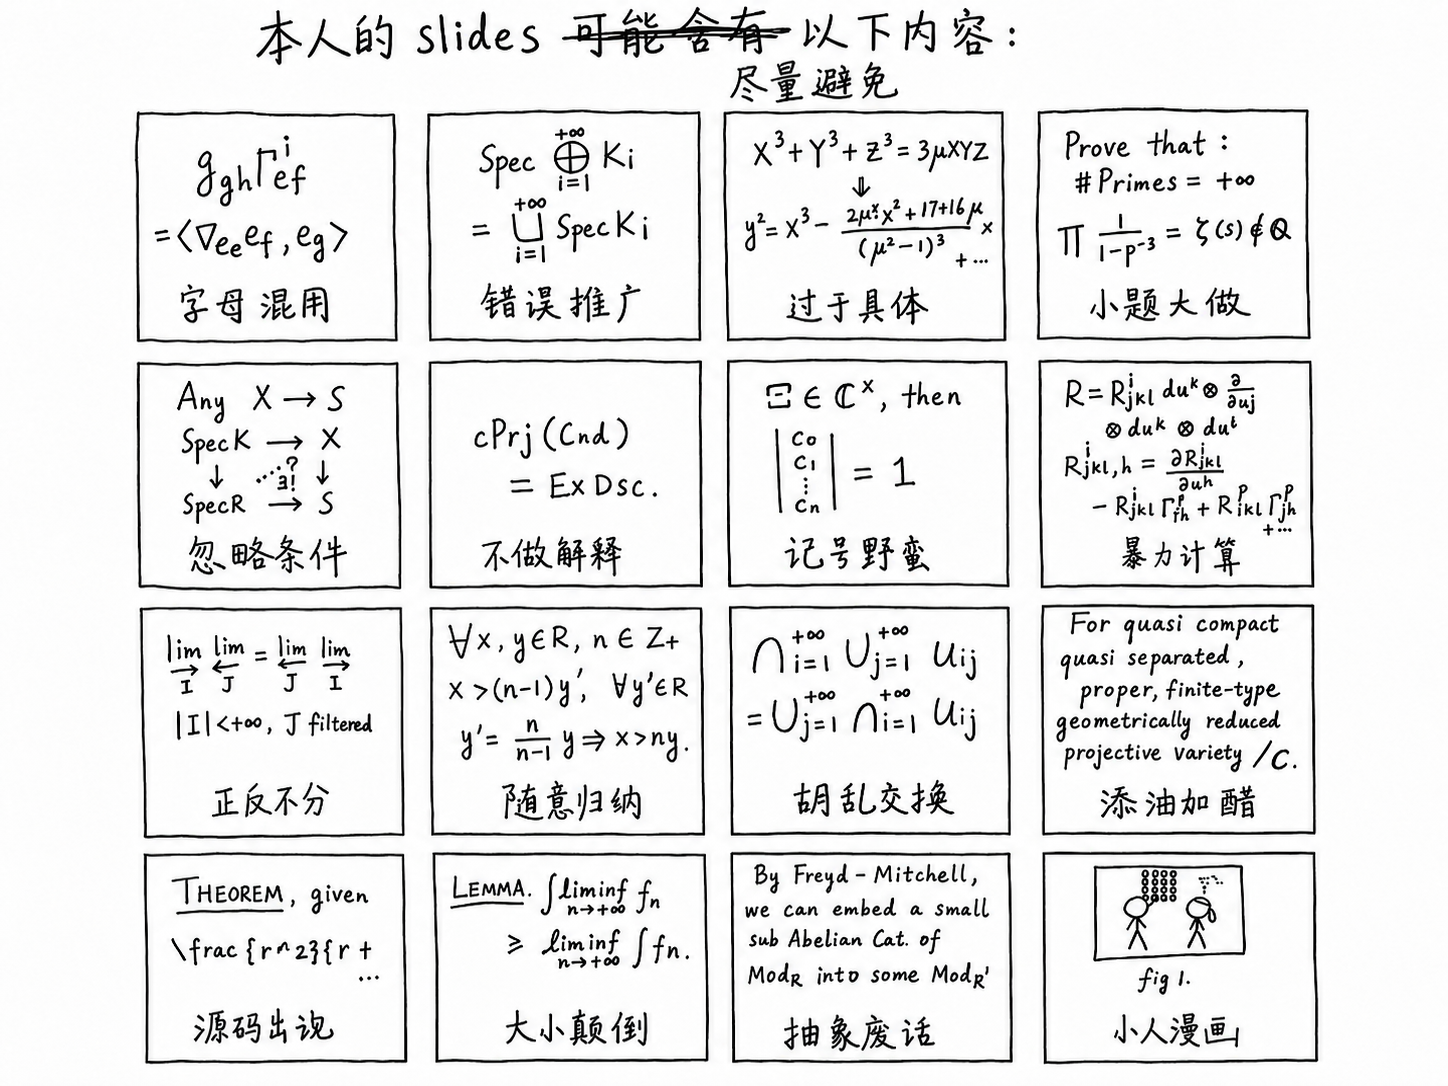
\includegraphics[width=\linewidth,height=.5\textheight,keepaspectratio]{figs/meme.png}
  \end{columns}
\end{frame}

\section{Motivation \& Background}

\begin{frame}{Predict-then-optimize v.s. Decision-focused learning}
  Given the covariance of $N$ assets' returns $\SigmaMat \in \RR^{N\times N}$, an investor often needs to solve a sparse portfolio optimization problem:
  \[ 
    \min_{\mathbf{w}\in\Wset_\Kcard} \mathbf{w}^\top \SigmaMat \mathbf{w},
    \qquad
    \Wset_\Kcard = \{\mathbf{w}\in\RR_+^N : \one^\top \mathbf{w}=1, \norm{\mathbf{w}}_0 \le k\} \tag{P}.
  \]

  \begin{columns}[T,onlytextwidth]
    \column{.48\linewidth}
    \textbf{Predict, then optimize}
    \begin{itemize}
      \item Decoupled. First use traditional statistical methods to estimate $\SigmaMat$, then solve the optimization problem.
      \item Trained for accuracy, not decision quality.
    \end{itemize}

    \column{.48\linewidth}
    \textbf{Decision-focused learning}
    \begin{itemize}
      \item End-to-end. Train the model parameters through the downstream optimization problem.
      \item E.g., Smart ``predict, then optimize'' \parencite{ElmachtoubGrigas2021SPO}.
    \end{itemize}
  \end{columns}

\end{frame}

\begin{frame}{Cardinality constraints Portfolio optimization}
  There are several ways of formulation to the problem
  \[
   \Wset_\Kcard = \{\mathbf{w}\in\RR_+^N : \one^\top \mathbf{w}=1, \norm{\mathbf{w}}_0 \le k\}.
   \]

By introducing binary indicators $z_i = \mathbb{I}\{w_i > 0\}$ to indicate if asset $i$ is included in the portfolio, the problem can be reformulated as a mixed-integer program (MIP):

\begin{itemize}
  \item \emph{Big-M formulation}: 
    \[
      \Wset_\Kcard^M
      =
      \left\{
        \mathbf{w}\in\RR_+^N,\; \mathbf{z}\in\{0,1\}^N :
        \one^\top \mathbf{w}=1,\;
        \one^\top \mathbf{z}=\Kcard,\;
        w_i \le z_i,\; i=1,\ldots,N
      \right\}.
    \] 
  \item \emph{Complementarity-type formulation} (tighter):
    \[
      \Wset_\Kcard^C
      =
      \left\{
        \mathbf{w}\in\RR_+^N,\; \mathbf{z}^c \in\{0,1\}^N :
        \one^\top \mathbf{w}=1,\;
        \one^\top \mathbf{z}^c=\Kcard,\;
        w_i z_i^c = 0,\; i=1,\ldots,N
      \right\}.
    \]
\end{itemize}
\end{frame}

\begin{frame}[allowframebreaks]{Factor Models in Finance}
\small

  \begin{itemize}
    \item Asset returns are modeled as \textbf{common factors} plus \textbf{idiosyncratic noise}:
      \[
        r_{it} = \alpha_i + \sum_{p=1}^P \beta_{ip} f_{pt} + \varepsilon_{it}
        \quad\Longleftrightarrow\quad
        \mathbf{R} = \one \boldsymbol{\alpha}^\top + \mathbf{F}\mathbf{B}^\top + \boldsymbol{\varepsilon}.
      \]
      Here $\mathbf{R}\in\RR^{T\times N}$, $\mathbf{F}\in\RR^{T\times P}$, $\boldsymbol{\alpha}\in\RR^N$, $\mathbf{B}\in\RR^{N\times P}$, and $\boldsymbol{\varepsilon}\in\RR^{T\times N}$.

    \item \textbf{Fama-French five-factor} model \parencite{FamaFrench2015FiveFactor}: \texttt{Mkt-Rf} (market risk premium), \texttt{SMB} (size), \texttt{HML} (value), \texttt{RMW} (profitability), and \texttt{CMA} (investment style).

    \item Factors are \emph{known, observable (at the end of the trade-day), and shared by all assets}; factor loadings $\beta_{ip}$ and idiosyncratic errors $\varepsilon_{it}$ are asset-specific:
      {
      \[
        \mathbf{F} =
        \begin{bmatrix}
          \texttt{Mkt-RF}_1 & \texttt{SMB}_1 & \texttt{HML}_1 & \texttt{RMW}_1 & \texttt{CMA}_1 \\
          \cdots & \cdots & \cdots & \cdots & \cdots \\
          \texttt{Mkt-RF}_T & \texttt{SMB}_T & \texttt{HML}_T & \texttt{RMW}_T & \texttt{CMA}_T
        \end{bmatrix}
        \in \RR^{T\times 5}.
      \] 
      }
      \end{itemize}
  \framebreak
  \small
    By denoting $\operatorname{Cov}(\mathbf{F}) := \SigmaMat_f \in \RR^{P\times P}$, $\operatorname{Cov}(\boldsymbol{\varepsilon}) := \boldsymbol{\Psi} \in \RR^{N\times N}$ (often assumed to be diagonal), and the asset covariance as $\SigmaMat \in \RR^{N\times N}$, and taking the covariance of the return model $\mathbf{R} = \one \boldsymbol{\alpha}^\top + \mathbf{F}\mathbf{B}^\top + \boldsymbol{\varepsilon}$ implies
    \[
      \SigmaMat = \mathbf{B} \SigmaMat_f \mathbf{B}^\top + \boldsymbol{\Psi} = \mathbf{B} \SigmaMat_f \mathbf{B}^\top + \diag(\psi_1^2, \ldots, \psi_N^2).
    \]
    \begin{block}{\small Remark}
          \begin{itemize}
            \small
            \vspace{0.4em}
          \item The factor covariance $\SigmaMat_f$ can be directly computed from the data.
          \item The parameters to be estimated are the factor loadings $\mathbf{B}$ and the idiosyncratic variances $\boldsymbol{\Psi}$.
          \item For convenience, one may collect the parameters into a single vector $\boldsymbol{\Param} = (\mathbf{B}, \boldsymbol{\Psi})$.
        \end{itemize}
    \end{block}
\end{frame}

% \begin{frame}{Cardinality constraints make the gap sharper}
%   A long-only sparse portfolio imposes
%   \[
%     \Wset_\Kcard
%     =
%     \left\{
%       \mathbf{w} \in \RR_+^{\Nassets} :
%       \norm{\mathbf{w}}_0 \le \Kcard,\;
%       \one^\top \mathbf{w} = 1
%     \right\}.
%   \]

%   \begin{itemize}
%     \item Choosing the support is combinatorial: there are $\binom{\Nassets}{\Kcard}$ possible subsets.
%     \item A small covariance-model error can change the selected support, not just the weights.
%     \item The induced map $\SigmaMat \mapsto w^\star(\SigmaMat)$ is discontinuous for the original MIP.
%   \end{itemize}

%   \begin{question}
%     If the downstream decision is discontinuous, what exactly should the prediction model learn?
%   \end{question}
% \end{frame}

% \begin{frame}{Positioning in decision-focused learning}
%   Decision-focused learning trains model parameters through the downstream optimizer:
%   \[
%     \min_\Param
%     \EE_{(X,Y)\sim\Dset}
%     \left[
%       \ell_d\!\left(\omega^\star(\Param,X),Y\right)
%     \right],
%     \qquad
%     \omega^\star(\Param,X)
%     =
%     \argmin_{\omega\in\Omega}
%     c\!\left(\omega,\xi(\Param,X)\right).
%   \]

%   \begin{itemize}
%     \item Continuous convex problems can be differentiated through KKT or cone-program sensitivity.
%     \item Existing combinatorial work mostly focuses on MILPs and cutting-plane relaxations.
%     \item This paper moves to a nonlinear convex quadratic MIP from sparse portfolio optimization.
%   \end{itemize}
% \end{frame}

% \begin{frame}{Paper's claim}
%   \begin{block}{One-sentence version}
%     Learn the factor risk model by back-propagating through a continuous relaxation of the cardinality-constrained portfolio optimizer, using realized Sharpe ratio as the decision-based training signal.
%   \end{block}

%   \begin{itemize}
%     \item Embed Big-M, SOCP, and SDP relaxations as differentiable decision layers.
%     \item Learn factor loadings and idiosyncratic risks jointly with the portfolio decision.
%     \item Compare against two decoupled baselines on S\&P 500 constituents.
%     \item Empirically, even the loose Big-M relaxation performs surprisingly well.
%   \end{itemize}
% \end{frame}

% \begin{frame}{Contributions to remember}
%   \begin{enumerate}
%     \item First end-to-end implementation, per the authors, for a nonlinear mixed-integer portfolio problem.
%     \item A DPP-compliant decision layer for sparse minimum-variance portfolios under factor covariance structure.
%     \item A comparison of relaxation tightness in learning: Big-M vs.\ SOCP vs.\ SDP.
%     \item Evidence that tighter relaxations do not automatically produce better learned decisions.
%   \end{enumerate}

%   \begin{discuss}{Reading angle}
%     The paper is as much about differentiable optimization design as it is about portfolio backtesting.
%   \end{discuss}
% \end{frame}

\section{Methodology}

\begin{frame}{Notation reference}
  \centering\small
  \begin{tabular}{>{\raggedright\arraybackslash}p{.28\linewidth}p{.65\linewidth}}
    
    \toprule
    Symbol & Meaning \\
    \midrule
    $\Nassets$, $\Kcard$ & number of assets, target cardinality \\
    $j \in \{1,\dots, J\}$ & problem instance index (for Bootstrap indexing) \\
    $\mathbf{w}\in\RR_+^\Nassets$ & long-only portfolio weights with $\one^\top \mathbf{w}=1$ \\
    $\mathbf{z}\in\{0,1\}^\Nassets, \tilde{\mathbf{{z}}} \in [0,1]^\Nassets$ & asset-selection indicators, continuous relaxation of $\mathbf{z}$ \\
    $\mathbf{F}^{(j)} \in \RR^{T \times P}$, $\mathbf{R}^{(j)} \in \RR^{T \times \Nassets}$ & factor returns, asset returns for problem instance $j$ \\
    $\mathbf{B}\in\RR^{\Nassets\times P}$ & factor loading matrix \\
    $\boldsymbol{\Psi}=\diag(\psi_1^2,\dots,\psi_\Nassets^2)$ & diagonal idiosyncratic covariance \\
    $\SigmaMat_f^{(j)} \in \RR^{P\times P}$ & sample covariance of factors in instance $j$ \\
    $\SigmaMat_\Param^{(j)} \in \RR^{\Nassets\times \Nassets}$ & model-implied asset covariance matrix ($\SigmaMat$ if non-paramterized) \\
    $\ell_d$ & decision-based realized loss \\
    \bottomrule
  \end{tabular}
\end{frame}

% \begin{frame}{Big-M cardinality formulation}
%   Introduce binary indicators $z_i$:
%   \[
%     z_i =
%     \begin{cases}
%       1, & \text{asset } i \text{ is included},\\
%       0, & \text{otherwise}.
%     \end{cases}
%   \]

%   The traditional feasible set is
%   \[
%     \Wset_\Kcard^M
%     =
%     \left\{
%       w\in\RR_+^\Nassets,\; z\in\{0,1\}^\Nassets :
%       \one^\top w=1,\;
%       \one^\top z=\Kcard,\;
%       w\le z
%     \right\}.
%   \]

%   \begin{itemize}
%     \item Advantage: simple linear constraints.
%     \item Problem: the continuous relaxation $0\le z\le 1$ is very loose under long-only budget constraints.
%   \end{itemize}
% \end{frame}

% \begin{frame}{Complementarity-type cardinality formulation}
%   A tighter alternative couples weights and indicators multiplicatively:
%   \[
%     \Wset_\Kcard^C
%     =
%     \left\{
%       w\in\RR_+^\Nassets,\; z\in\{0,1\}^\Nassets :
%       \one^\top w=1,\;
%       \one^\top z=\Kcard,\;
%       w\odot(\one-z)=0
%     \right\}.
%   \]

%   The paper also uses the complement indicators $z^c$:
%   \[
%     \Wset_\Kcard^{C'}
%     =
%     \left\{
%       w\in\RR_+^\Nassets,\; z^c\in\{0,1\}^\Nassets :
%       \one^\top w=1,\;
%       \one^\top z^c=\Nassets-\Kcard,\;
%       w\odot z^c=0
%     \right\}.
%   \]

%   \begin{remark}
%     These formulations have tighter relaxations, but the continuous complementarity version is degenerate.
%   \end{remark}
% \end{frame}

% \begin{frame}{Nominal sparse minimum-variance portfolio}
%   The generic deterministic problem is
%   \[
%     \pi^\star(\xi) := \min_{\omega\in\Omega} c(\omega,\xi).
%   \]

%   In this paper:
%   \[
%     \pi^\star(\SigmaMat)
%     :=
%     \min_{w\in\Wset_\Kcard}
%     w^\top \SigmaMat w.
%     \tag{$P_{mV}$}
%   \]

%   \begin{itemize}
%     \item Decision variable: portfolio weights $w$.
%     \item Parameter: asset covariance matrix $\SigmaMat$.
%     \item Objective: ex-ante portfolio variance.
%     \item Constraint: long-only, budgeted, sparse support.
%   \end{itemize}
% \end{frame}

% \begin{frame}{Linear factor covariance model}
%   \small
%   The asset-return model is
%   \[
%     r_{it}
%     =
%     \alpha_i
%     +
%     \sum_{p=1}^{P}
%     \beta_{ip} f_{pt}
%     +
%     \varepsilon_{it},
%     \qquad
%     r_t = \alpha + B f_t + \varepsilon_t.
%   \]

%   With diagonal residual covariance
%   \[
%     \Psi = \diag(\psi_1^2,\ldots,\psi_\Nassets^2),
%   \]
%   the covariance estimate becomes
%   \[
%     \SigmaMat(B,\Psi;\SigmaMat_f)
%     =
%     B\SigmaMat_f B^\top + \Psi.
%   \]

%   \begin{block}{Decision relevance}
%     The model parameters are estimated at the asset level, but the loss that matters is portfolio-level.
%   \end{block}
% \end{frame}

\subsection{Predict, then optimize baseline}

\begin{frame}{LinReg: Decoupled baseline (predict, then optimize)}
  \small 
  \begin{algorithm}[H]
    \DontPrintSemicolon
    \KwIn{Factors $\mathbf{F}^{(j)}$, returns $\mathbf{R}^{(j)}$, cardinality $k$}
    Fitting the factor model $\mathbf{R} = \one \boldsymbol{\alpha}^\top + \mathbf{F}\mathbf{B}^\top + \boldsymbol{\varepsilon}$ directly on accuracy accuracy loss $\ell_a$ to obtain $\hat{\boldsymbol{\Param}}^{(j)}= (\hat{\mathbf{B}}^{(j)}, \hat{\boldsymbol{\Psi}}^{(j)})$    .\;
    Construct the covariance $\SigmaMat_{\hat{\Param}}^{(j)} = \hat{\mathbf{B}}^{(j)} \SigmaMat_f^{(j)} \hat{\mathbf{B}}^{(j)\top} + \hat{\boldsymbol{\Psi}}^{(j)}$.\;
    Solve the cardinality-constrained problem with by solver: $\mathbf{w}^{(j)}:=\argmin_{\mathbf{w}\in\Wset_\Kcard} \mathbf{w}^\top \SigmaMat_{\hat{\Param}}^{(j)} \mathbf{w}$.\;
    \KwOut{Portfolio weights $\mathbf{w}^{(j)}$}
  \end{algorithm}

  \begin{itemize}
    \item Accuracy loss does not see the sparse optimizer.
    \item The fitted covariance is treated as deterministic.
    \item Mean-variance portfolios are highly sensitive to estimation error.
  \end{itemize}
\end{frame}

\subsection{End-to-end framework}

% \begin{frame}{General bilevel learning objective}
%   \small 
%   For a mini-batch $\Bset^{(m)}$, train the risk-model parameters
%   $\Param=\{\mathbf B,\boldsymbol{\Psi}\}$ by
%   \[
%     \min_{\Param}\;
%     \Loss^{(m)}(\Param)
%     =
%     \frac{1}{|\Bset^{(m)}|}
%     \sum_{j\in\Bset^{(m)}}
%     \ell_d\!\left(\mathbf w_j^\star,\mathbf R^{(j)}\right)
%   \]
%   subject to, for each $j\in\Bset^{(m)}$,
%   \[
%     \mathbf w_j^\star
%     \in
%     \argmin_{\mathbf w\in\Wset_\Kcard}
%     \mathbf w^\top \SigmaMat_\Param^{(j)} \mathbf w,
%     \qquad
%     \SigmaMat_\Param^{(j)}
%     =
%     \mathbf B\SigmaMat_f^{(j)}\mathbf B^\top+\boldsymbol{\Psi}.
%   \]

%   \begin{itemize}
%     \item Inner problem: solve the sparse minimum-variance portfolio using
%       $\SigmaMat_\Param^{(j)}$.
%     \item Outer problem: update $\Param$ to reduce realized decision loss.
%   \end{itemize}
% \end{frame}

\begin{frame}{End-to-End architecture as a computational graph}
  \centering
  \makebox[\textwidth][c]{%
  \resizebox{1.12\textwidth}{!}{%
  \begin{tikzpicture}[
    >=Latex,
    font=\small,
    basebox/.style={
      rounded corners=2pt,
      line width=.65pt,
      align=center,
      inner xsep=5pt,
      inner ysep=4pt,
      minimum height=11mm
    },
    data/.style={basebox, draw=blue!55!black, fill=blue!4, text width=28mm},
    model/.style={basebox, draw=orange!70!black, fill=orange!6, text width=33mm},
    covbox/.style={basebox, draw=orange!70!black, fill=orange!6, text width=42mm},
    opt/.style={basebox, draw=green!50!black, fill=green!5, text width=51mm},
    loss/.style={basebox, draw=red!60!black, fill=red!5, text width=38mm},
    signal/.style={basebox, draw=black!55, fill=black!3, text width=34mm},
    flow/.style={-{Latex[length=2.1mm]}, draw=black!85, line width=.95pt},
    train/.style={-{Latex[length=2.1mm]}, draw=black!85, dashed, line width=.95pt},
    lab/.style={font=\scriptsize, align=center, inner sep=.4pt, text=black}
  ]
    \node[data] (sample) at (-2.0,0) {
      Training sample $j$\\[.6mm]
      $\{\mathbf F_j,\mathbf R_j\}$
    };

    \node[model] (risk) at (5.4,-3.05) {
      Risk model\\[.6mm]
      $\boldsymbol{\Param}=\{\mathbf B,\Psi\}$\\
      {\tiny trainable parameters}
    };

    \node[covbox] (cov) at (5.4,0) {
      Covariance\\[.6mm]
      $\widehat{\mathbf\Sigma}_j
      =
      \mathbf B\widehat{\mathbf\Sigma}_{f,j}\mathbf B^\top+\Psi$
    };

    \node[opt] (solver) at (18.7,0) {
      Differentiable optimization layer\\[.6mm]
      $\displaystyle
      \mathbf w_j^\star
      =
      \arg\min_{\mathbf w\in\mathcal W_k}
      \mathbf w^\top
      \widehat{\mathbf\Sigma}_j
      \mathbf w$
    };

    \node[loss] (loss) at (18.7,-3.05) {
      Realized decision loss\\[.6mm]
      $\ell_j=\ell_d(\mathbf w_j^\star,\mathbf R_j)$
    };

    \node[signal] (update) at (11.6,-3.05) {
      Backward update\\[.6mm]
      $\nabla_\Param \ell_j$\\
      {\tiny implicit / surrogate gradient}
    };

    % \draw[flow] (sample) -- node[above=2pt, lab] {input\\factors} (risk);
    \draw[flow] (risk) -- node[pos=.55, right=2pt, lab, align=left] {learned\\parameters} (cov);
    \draw[flow] (cov) -- node[above=2pt, lab] {predicted\\covariance} (solver);
    \draw[flow] (solver) -- node[pos=.55, right=2pt, lab, align=left] {optimal\\portfolio} (loss);
    \draw[flow] (loss) -- node[above=2pt, lab] {gradient\\signal} (update);
    \draw[train] (update) -- node[above=4pt, lab] {update $\Param$} (risk);
    \draw[flow] (sample.south) -- ++(0,-4.55) coordinate (returnbase)
      -- (returnbase -| loss.south) coordinate (returncorner)
      -- (loss.south);
    \node[lab, align=left, anchor=south east, xshift=-2pt, yshift=2pt] at (returncorner)
      {realized returns $\mathbf R_j$};
    \draw[flow] (sample.east) -- node[above=2pt, lab] {estimate $\widehat{\mathbf\Sigma}_{f,j}$} (cov.west);
  \end{tikzpicture}
  }%
  }
\end{frame}


\begin{frame}{Limitation of current MIP formulation \& relaxation layers}
    \small 
The dependency $\ell_d\!\left(\argmin_{\mathbf{w}\in\Wset_\Kcard}\mathbf{w}^\top \SigmaMat_\Param \mathbf{w},\mathbf{R}\right)$ creates two obstacles:

{\addtolength{\leftmargini}{1em}
\begin{enumerate}
  \item $\Wset_\Kcard$ is discrete; the optimizer jumps between supports.
  \item Even for continuous problems, differentiating $\argmin$ requires sensitivity analysis.
\end{enumerate}
}

Thus, consider the following three possible continuous convex relaxations to remove discreteness:
\vspace{1em}

{
\centering
\begin{tabular}{>{\raggedright\arraybackslash}p{.2\linewidth}
                >{\raggedright\arraybackslash}p{.44\linewidth}}
  \toprule
  Layer & Main tradeoff \\
  \midrule
  E2E M & Loosest but computationally cheapest \\
  E2E SOCP \cite{CuiZhengZhuSun2013Relaxations} & Tighter; conic constraints add cost \\
  E2E SDP \cite{WiegeleZhao2022SDP} & Tightest target; much larger decision layer \\
  \bottomrule
\end{tabular}
\par
}

\end{frame}

\begin{frame}[allowframebreaks]{E2E Big-M relaxation}
  \small 
  For instance $j$, the Big-M relaxation layer solves
  \[
  \begin{aligned}
    \min_{\mathbf w,\tilde{\mathbf z}}\quad 
    &  \mathbf w^\top \mathbf{B} \SigmaMat_f^{(j)} \mathbf{B}^\top \mathbf{w} + \mathbf{w}^\top \boldsymbol{\Psi} \mathbf{w}
    \end{aligned}
  \]
  subject to
  \[
  \begin{aligned}
    & \one^\top \mathbf w=1,\qquad
      \one^\top \tilde{\mathbf z}\le \Kcard,\qquad
      \mathbf w\le \tilde{\mathbf z},\\
    & 0\le \tilde{\mathbf z}\le \one,\qquad
      \mathbf w\ge0,
  \end{aligned}
  \]

  \begin{remark}
    \vspace{0.4em}
      \begin{itemize}
      \item $\tilde{\mathbf z}\in[0,1]^\Nassets$ is the continuous relaxation of indicators $\mathbf{z}\in\{0,1\}^\Nassets$.
      \item Note that $\one^\top \tilde{\mathbf z}\le \Kcard$ is now a soft constraint, so the solution may have more than $k$ nonzeros.
      \item Empirically, this loose layer is the fastest and often performs best.
  \end{itemize}
    
  \end{remark}
  
  \break

  Moreover, note that the idiosyncratic risk term $\boldsymbol{\Psi}$ is a diagonal matrix with positive entries. Thus, to keep this specific structure during gradient updates, the actual updated parameter is
  \[
    \hat{\boldsymbol{\psi}} = [\hat{\psi}_1,\ldots,\hat{\psi}_\Nassets]^\top,
    \]
  and the final idiosyncratic covariance is given by
  \[
    \boldsymbol{\Psi} = 
      \diag\!\left(\psi_1^2,\ldots,\psi_\Nassets^2\right)
    := \begin{pmatrix}
      \exp(\hat{\psi}_1)^2  & \cdots & 0 \\
      \vdots  & \ddots & \vdots \\
      0  & \cdots & \exp(\hat{\psi}_\Nassets)^2
    \end{pmatrix}.
  \]

  This is also the case for the remaining two relaxations.


\end{frame}

\begin{frame}{E2E SOCP relaxation}
  \small
  The SOCP relaxation separates systematic and idiosyncratic risk:
  \[
    \min_{\mathbf{w},\tilde{\mathbf z},\boldsymbol{\delta}}
    \mathbf{w}^\top \mathbf{B}\SigmaMat_f \mathbf{B}^\top \mathbf{w}
    + \diagv(\Psi)^\top\boldsymbol{\delta}
  \]
  subject to
  \[
  \begin{aligned}
    &\one^\top \mathbf{w}=1,\quad
      \one^\top \tilde{\mathbf z}\le \Kcard,\quad
      \mathbf{w}\le \tilde{\mathbf z},\quad
      w_i^2 \le \delta_i \tilde z_i ~(\forall i),  \quad 0\le\tilde{\mathbf z}\le\one,\quad
      \mathbf{w}\ge0,\quad
      \boldsymbol{\delta}\ge0.
  \end{aligned}
  \]

\begin{block}{\small Intuition of $\delta_i$}
  \footnotesize
      \vspace{0.4em}
  \begin{itemize}
    \item Consider a toy model: $\min_w \psi^2 w^2$, s.t., $\psi^2 > 0$. By introducing $\delta$ and get $\min_{w,\delta} \psi^2 \delta$, s.t., $w^2 \le \delta$. The optimal solution is $\delta^\star = w^{\star 2}$, and the objective value is $\psi^2 w^{\star 2}$, which is the same as the original problem.
    \item Then consider $w_i^2 \le \delta_i z_i$ with $z_i \in \{0,1\}$. If $z_i=1$, then $w_i^2 \le \delta_i$ and it is the same as the toy model. If $z_i=0$, then $w_i^2 \le 0$ implies $w_i=0$, which is consistent with the original problem.
    \item For relaxed term when $\tilde z_i \in (0,1)$, the constraint $\delta_i \geq w_i^2/\tilde z_i > w_i^2$. It imposes a stronger penalty on $\delta_i$ than the original problem, which encourages $\tilde z_i$ to be close to 0 or 1, and discourages fractional solutions (hesitant solutions).
  \end{itemize}
\end{block}
\end{frame}

\begin{frame}{E2E SDP relaxation layer}
  \footnotesize
  \setlength{\abovedisplayskip}{0.35em}
  \setlength{\belowdisplayskip}{0.35em}
  The SDP reformulation is
  \[
    \min_\mathbf{U} \; \left\langle \SigmaMat_\Param, \mathbf{W} \right\rangle
  \]
  subject to
  \[
  \begin{aligned}
    \one^\top \mathbf{w} =1,\quad \one^\top \mathbf{\tilde z}^c=\Nassets-\Kcard, \quad \mathbf{w}, \mathbf{\tilde z}^c \ge 0, \quad
    \diagv(\mathbf{\tilde Z}^c) =\mathbf{\tilde z}^c,
    \quad
    \diagv(\mathbf{Q})=0,\quad
    \mathbf{U}  =
    \begin{pmatrix}
      1 & \mathbf{w}^\top & \mathbf{\tilde z}^{c\top}\\
      \mathbf{w} & \mathbf{W} & \mathbf{Q}\\
      \mathbf{\tilde z}^c & \mathbf{Q}^\top & \mathbf{\tilde Z}^c
    \end{pmatrix}   \succeq 0.
  \end{aligned}
  \]

  \only<1>{%
    \begin{block}{\footnotesize (Very naive) Intuition of $\mathbf{U} \succeq 0$}
    \begin{itemize}
      \scriptsize
      \setlength{\itemsep}{0.1em}
      \item  According to the Schur complement condition, $\mathbf{U} \succeq 0$ is equivalent to $\begin{pmatrix}
        \mathbf{W} - \mathbf{w}\mathbf{w}^\top & \mathbf{Q} - \mathbf{w}\mathbf{\tilde z}^{c\top}\\
        \mathbf{Q}^\top - \mathbf{\tilde z}^c \mathbf{w}^\top & \mathbf{\tilde Z}^c - \mathbf{\tilde z}^c \mathbf{\tilde z}^{c\top}
      \end{pmatrix}\succeq 0$. This means that the lifted variables $\mathbf{W}$, $\mathbf{\tilde Z}^c$, and $\mathbf{Q}$ are consistent with the original variables $\mathbf{w}$ and $\mathbf{\tilde z}^c$ in a positive semidefinite sense.
      \item Or equivalently, for exact lifted solutions, one hopes $\mathbf{U}_{\text{exact}} :=
      \begin{pmatrix}
        1 & \mathbf{w}^\top & \mathbf{\tilde z}^{c\top}\\
        \mathbf{w} & \mathbf{W} & \mathbf{Q}\\
        \mathbf{\tilde z}^c & \mathbf{Q}^\top & \mathbf{\tilde Z}^c
      \end{pmatrix} = \begin{pmatrix}
        1 & \mathbf{w}^\top & \mathbf{\tilde z}^{c\top}\\
        \mathbf{w} & \mathbf{w}\mathbf{w}^\top & \mathbf{w}\mathbf{\tilde z}^{c\top}\\
        \mathbf{\tilde z}^c & \mathbf{\tilde z}^c \mathbf{w}^\top & \mathbf{\tilde z}^c \mathbf{\tilde z}^{c\top}
      \end{pmatrix}$, which mathematically implies $\mathbf{U}_{\text{exact}} \succeq 0$ and $\operatorname{rank}(\mathbf{U}_{\text{exact}}) = 1$. The SDP relaxation drops the rank-1 constraint (as it is non-convex), but the PSD constraint still encourages low-rank solutions.
      \item To conclude with, the PSD constraint $\mathbf{U} \succeq 0$ implies that $\mathbf{W} \approx \mathbf{w}\mathbf{w}^\top$, $\mathbf{\tilde Z}^c \approx \mathbf{\tilde z}^c \mathbf{\tilde z}^{c\top}$, and $\mathbf{Q} \approx \mathbf{w}\mathbf{\tilde z}^{c\top}$, which is the key to the tightness of the SDP relaxation.
    \end{itemize}
  \end{block}
  }

  \only<2>{%
  \begin{block}{\footnotesize Intuition of the objective}
    \footnotesize
    \begin{itemize}
      \setlength{\itemsep}{0.1em}
          \vspace{0.4em}
      \item  Still consider the exact term $\mathbf{W} = \mathbf{w}\mathbf{w}^\top$. Then the original objective $\mathbf{w}^\top \SigmaMat_\Param \mathbf{w} = \operatorname{Tr}(\SigmaMat_\Param \mathbf{w}\mathbf{w}^\top) = \left\langle \SigmaMat_\Param, \mathbf{W} \right\rangle$.
      \item Thus, current version is an approximate lifted surrogate for $\mathbf{w}\mathbf{w}^\top$.
    \end{itemize}
  \end{block}
  }

  \only<3>{%
  \begin{block}{\footnotesize Intuition of the constraints w.r.t. $\mathbf{Z}^c$ }
    \footnotesize
    \begin{itemize}
      \setlength{\itemsep}{0.1em}
          \vspace{0.4em}
      \item For exact lifted solutions with binary indicators $\mathbf{Z}_{\text{exact}}^c = \mathbf{z}^c \mathbf{z}^{c\top}$, its diagonal entries are $(\mathbf{Z}_{\text{exact}}^c)_{ii} = z_i^c z_i^c = z_i^c$, i.e. $\diagv(\mathbf{Z}_{\text{exact}}^c) = \mathbf{z}^c$.  In the relaxed case, we keep this necessary condition $\diagv(\mathbf{\tilde Z}^c) = \mathbf{\tilde z}^c$, without enforcing the full rank-1 constraint $\mathbf{\tilde Z}^c = \mathbf{\tilde z}^c \mathbf{\tilde z}^{c\top}$.
      \item Furthermore, $\mathbf{U} \succeq 0$ implies $\mathbf{\tilde Z}^c - \mathbf{\tilde z}^c \mathbf{\tilde z}^{c\top} \succeq 0$, which means $(\mathbf{\tilde Z}^c)_{ii} \ge (\mathbf{\tilde z}^c)_i^2$ for all $i$. Given that $(\mathbf{\tilde Z}^c)_{ii} = (\mathbf{\tilde z}^c)_i$, we have $(\mathbf{\tilde z}^c)_i \ge (\mathbf{\tilde z}^c)_i^2$, which implies $(\mathbf{\tilde z}^c)_i \in [0,1]$ for all $i$. Thus, the box constraint $0 \le \mathbf{\tilde z}^c \le \one$ is inherent in $\mathbf{U} \succeq 0$.
    \end{itemize}
  \end{block}
  }

  \only<4>{%
  \begin{block}{\footnotesize Intuition of the constraints w.r.t. $\mathbf{Q}$ }
    \footnotesize
    \begin{itemize}
      \setlength{\itemsep}{0.1em}
          \vspace{0.4em}
      \item Similarly, for binary indicators, the original complementarity constraint is $w_i z_i^c = 0$ for all $i$. Thus in the exact lifted case, we have $\mathbf{Q}_{\text{exact}} = \mathbf{w}\mathbf{\tilde z}^{c\top}$, and $w_i z_i^c = 0$ implies $\diagv(\mathbf{Q}_{\text{exact}}) = \mathbf{0}$.
      \item In the relaxed case, the PSD condition gives $(\mathbf{W}_{ii} - w_i^2) {\tilde z^c_i} (1-\tilde z^c_i) \geq w_i^2 (\tilde z_i^c)^2$ for all $i$.
      \begin{itemize}
        \scriptsize
        \setlength{\itemsep}{0.05em}
            \vspace{0.4em}
        \item For $\tilde z^c_i = 1$, the constraint reduces to $\mathbf{W}_{ii} \geq w_i^2$, which is consistent with the original problem.
        \item For $\tilde z^c_i = 0$, the constraint reduces to $\mathbf{W}_{ii} \geq 0$, which does not impose any additional restriction on $w_i$ since $w_i \geq 0$ is already a constraint.
        \item For $\tilde z^c_i \in (0,1)$, the constraint becomes $\mathbf{W}_{ii} \geq \frac{w_i^2}{1 - \tilde z_i^c}$, which is a stronger constraint than the original problem, and it encourages $\tilde z_i^c$ to be close to 0 or 1, and discourages fractional solutions (hesitant solutions).
      \end{itemize}
    \end{itemize}
  \end{block}
  }

\end{frame}



\begin{frame}{DPP compliance}
  \small
  \texttt{CvxPyLayers} \parencite{AgrawalAmosEtAl2019Layers} is a library for differentiating through convex optimization problems. It requires the problem to comply with DPP (Disciplined Parametrized Programming). As long as the problem is DPP-compliant, the library can automatically solve the optimization problem in forward passes and compute gradients in backward passes.
  \begin{itemize}
    \small
    \item For SOCP, the paper introduces artificial variables
  \[
    \mathbf{v} = \mathbf{B}^\top \mathbf{w},\qquad
    \bar{\mathbf{v}} = \SigmaMat_f^{1/2}\mathbf{v},
  \]
  and the objective can be rewritten as 
  \[ \min \|\bar{\mathbf{v}}\|_2^2 + \diagv(\Psi)^\top\boldsymbol{\delta}.\]

  \item For SDP, define 
  \[
    \mathbf{\bar{V}} := \mathbf{W} \mathbf{B}, \qquad \mathbf{V} := \mathbf{B}^\top \mathbf{\bar{V}}.
    \]  
    Then the objective can be rewritten as 
    \[ \min \langle \SigmaMat_f, \mathbf{V} \rangle + \langle \boldsymbol{\Psi}, \mathbf{W} \rangle,\]
  \end{itemize}

\end{frame}

\begin{frame}{Forward pass}
    \small 
  For each instance $j$:
  \begin{enumerate}
    \item Compute factor covariance $\SigmaMat_f^{(j)}$.
    \item Build the risk-model parameters
    \[
      \SigmaMat_\Param^{(j)}
      =
      \mathbf{B}\SigmaMat_f^{(j)}\mathbf{B}^\top
      +
      \diag\!\left(\exp(\hat\psi)^2\right).
    \]
    \item Solve the selected DPP-compliant relaxation.
    \item Return relaxed portfolio weights $\mathbf w^{\star(j)}$.
  \end{enumerate}

\end{frame}

\begin{frame}{Loss function}
  \small 

  \begin{itemize}
  \item  After obtaining the optimal portfolio weights $\mathbf w^{\star(j)}$ for instance $j$, we can then compute the portfolio's realized return $\mathbf{r}_{\text{p}^{(j)}} = \mathbf w^{\star(j)\top} \mathbf R^{(j)} \in \RR^T$ and evaluate its performance.

  % \item  In some other decision-focused learning problems, the loss is a regret-type or realized decision loss. However, either one requires the true covariance $\SigmaMat^\star$, yet it is not observable in stock return data. 

  \item  The paper chooses to directly use the annualized Sharpe ratio:
  \[
    \ell_d^{(j)}
    =
    \frac{(1+\mu(\mathbf{r}_{\text{p}^{(j)}}))^{365}}
         {\sqrt{256}\,\sigma(\mathbf{r}_{\text{p}^{(j)}})}.
  \]
  where $\mu(\mathbf{r}_{\text{p}^{(j)}})$ is the geometric mean, and $\sigma(\mathbf{r}_{\text{p}^{(j)}})$ is the standard deviation, with the annualization factor of $365$ and $256$ trading days, respectively. Further assume risk-free rate $r_f = 0$ for simplicity. Larger sharpe ratio means better performance.

  \item For the training batch, the loss is averaged across instances with negative sign:
  \[
    \Loss^{(m)} = -\frac{1}{|\Bset^{(m)}|} \sum_{j\in\Bset^{(m)}} \ell_d^{(j)}.
  \]

  \end{itemize}
\end{frame}

\begin{frame}{Backward pass}
\footnotesize
  \setlength{\abovedisplayskip}{0.35em}
  \setlength{\belowdisplayskip}{0.35em}
  During the backward pass, the goal is to compute the gradient $\grad_\Param \Loss^{(m)}$ to update the risk-model parameters $\Param$ via SGD, where 
  \[
    \grad_\Param \ell_d^{(j)}
    =
    \frac{\partial \ell_d^{(j)}}{\partial \mathbf{w}}
    \frac{\partial \mathbf{w}}{\partial \Param}.
  \]

  \begin{itemize}
    \setlength{\itemsep}{0.15em}
    \item $\partial \ell_d/\partial \mathbf{w}$ can be explicitly computed by the chosen loss function, e.g., Sharpe ratio.
    \item $\partial \mathbf{w}/\partial\Param$ is the harder part, which is here automatically done by \texttt{CvxPyLayers} \parencite{AgrawalAmosEtAl2019Layers}.
  \end{itemize}

  \begin{block}{\footnotesize Intuition of differentiating through optimization}
    \footnotesize
        \vspace{0.4em}
    Generally, given some optimization problem $\mathbf{w}^\star \in \argmin P_\Param(\mathbf{w})$ as part of a neural network.
    \begin{itemize}
      \setlength{\itemsep}{0.1em}
      \item It means that $\Param$ defines an optimization problem, and the solver returns the optimal solution $\mathbf{w}^\star$. 
      \item Under some regularity conditions, this optimization problem is differentiable, can be backpropagated through.
      \item Roughly, since $\mathbf{w}^\star$ is the optimal solution, it must satisfy some optimality conditions $F$, e.g., KKT conditions, which contain $\Param$ and $\mathbf{w}^\star$ simultaneously. Then by implicit differentiation,
      \[
       \frac{\partial \mathbf{w}^\star}{\partial \Param} = -\left(\frac{\partial F}{\partial \mathbf{w}^\star}\right)^{-1} \frac{\partial F}{\partial \Param}.
      \]
    \end{itemize}
  \end{block}
\end{frame}

\begin{frame}{Algorithm 2: E2E learning procedure}
  \scriptsize
  \begin{algorithm}[H]
    \DontPrintSemicolon
    \KwIn{learning rate $\gamma$, schedule, batch size $b$, epochs}
    \KwData{factors $\mathbf F^{(j)}$ and returns $\mathbf R^{(j)}$, $j=1,\ldots,J$}
    Initialize parameters $\boldsymbol{\Param}=\{\mathbf B,\hat\psi\}$.\;
    Distribute instances into mini-batches $\Bset^{(m)}$.\;
    \For{each epoch}{
      \For{each batch $\Bset^{(m)}$}{
        \For{each $j\in\Bset^{(m)}$}{
          compute $\SigmaMat_{\boldsymbol{\Param}}^{(j)}$ using $\mathbf F^{(j)}$ and current $\boldsymbol{\Param}$\;
          solve the relaxation layer and obtain $\mathbf{w}^{\star(j)}$\;
          compute instance loss $\ell_d(\mathbf{w}^{\star(j)},\mathbf{R}^{(j)})$\;
        }
        average batch loss $\Loss^{(m)}$ and update
        $\boldsymbol{\Param}\leftarrow\boldsymbol{\Param}-\gamma\grad_{\boldsymbol{\Param}} \Loss^{(m)}$\;
      }
    }
    Use trained $\boldsymbol{\Param}^\star$ to build the test-time covariance and solve the original sparse portfolio problem.\;
  \end{algorithm}
\end{frame}

\section{Experiments}

\subsection{Experimental setup}

\begin{frame}{Data and backtest design}
    \small 
  \begin{itemize}
    \item Assets: $\Nassets=50$ S\&P 500 constituents across GICS sectors.
    \item Factors: Fama--French five factors \cite{FamaFrench2015FiveFactor}.
    \item Cardinality levels: $\Kcard\in\{10,15,20\}$.
    \item Date range: daily prices from 2010--2021.
    \item Training window: previous five years of weekly returns.
    \item Rebalancing: every three months; out-of-sample period 2015--2021.
    \item Comparison: E2E-M, E2E-SOCP, E2E-SDP, decoupled factor model (linReg), and nominal model (directly estimate covariance from data).
  \end{itemize}
\end{frame}

\begin{frame}[allowframebreaks]{Circular block bootstrap \parencite{PolitisRomano1991CBB} for training data generation}
  \small 

  \emph {Why more data?}

  \begin{itemize}
    \item For each training period, original there is only one piece of data $\mathbf{R} \in \RR^{T\times \Nassets}$, $\mathbf{F} \in \RR^{T\times P}$, and is not sufficient for E2E methods to train $\boldsymbol \Param$.
    \begin{itemize}
      \small
      \item  For example, standing at 2015/01/01, the only available data is the weekly returns of 50 stocks and 5 factors from 2010/01/01 to 2014/12/31. Simulation is needed to generate more data for training.
    \end{itemize}
    \item Note that during training, the data frequency is weekly. Daily data is more abundant, but it may contains more noise, more complex dynamics and instationarity.
    \item Also, a five-year window is also a common practice. With approximately $5\times 52 = 260$ weekly data points, it is also a trade-off.
  \end{itemize}

  \break

  \emph{How to cicularly bootstrap?}
  \begin{itemize}
    \footnotesize
    \item Genearlly, given a time series of length $T$: $X_{1:T}$, first choose a block size $b$ and then slice the original time series into $k = T/b$ blocks, i.e., 
    \[
        X_{1:T} = [X_{1:b}, X_{b+1:2b}, \ldots, X_{(k-1)b+1:kb}] = [B_1, B_2, \ldots, B_k]
      \]
    \item Then for bootstrapping, randomly sample $k$ blocks with replacement from $\{B_1,\ldots,B_k\}$ and concatenate them to get a bootstrapped time series of length $T$: 
    \[\tilde{X}_{1:T}^{(j)} = [\tilde{B}_1^{(j)}, \tilde{B}_2^{(j)}, \ldots, \tilde{B}_k^{(j)}].\]

    \item The circular block bootstrap preserves the temporal dependence structure within each block, and by sampling blocks with replacement, it can generate new time series that are similar to the original one but with some randomness, which is useful for training the E2E model.

    \item In the paper, the block size is chosen as $b=20$ weeks, and the paper generates $J=2000$ bootstrapped time series for training.
  \end{itemize}


\end{frame}

\begin{frame}{Detailed training procedure}
  \footnotesize
  \only<1>{%
  \begin{itemize}
    \item For each training, a five-year window of weekly returns is used to train the E2E model (e.g., the first training period is 2010Q1 $\sim$ 2014Q4). With such many data (and by bootstrapping), the paper will compute the factor covariance $\SigmaMat_f^{(j)}$ for each instance $j$ and then train the E2E model by SGD to get the optimal parameters $\Param^\star$.
  \end{itemize}
  }

  \only<2>{%
  \begin{itemize}

    \item After training, the paper will use the trained $\Param^\star$ to build the test-time covariance $\SigmaMat_{\Param^\star}$ and solve the original sparse portfolio problem
      \[
        \min_{\mathbf{w}\in\Wset_\Kcard} \mathbf{w}^\top \SigmaMat_{\Param^\star} \mathbf{w}.
      \]
      directly by Gurobi to get the final portfolio weights $\mathbf{w}^\star$ for out-of-sample evaluation.

  \end{itemize}
  }

  \only<3>{%
  \begin{itemize}

    \item During evaluation, the model will buy-and-hold the portfolio for three months to get the realized return $\mathbf{r}_{\text{p}} \in \RR^T$ and compute the performance metrics, e.g., annualized return, volatility, Sharpe ratio, max drawdown, etc.

  \end{itemize}
  }

  \only<4>{%
  \begin{itemize}
    \item This procedure is repeated for every three months from 2015 to 2021 (so the next training period is 2010Q2 $\sim$ 2015Q1 and evaluate on 2015Q2), and the paper will report the average performance across all these out-of-sample periods.
  \end{itemize}
  }

    \begin{center}
    \resizebox{.90\textwidth}{!}{%
    \begin{tikzpicture}[
      font=\sffamily,
      title/.style={font=\sffamily\scriptsize},
      rowlab/.style={font=\sffamily\scriptsize},
      dots/.style={font=\sffamily\scriptsize}
    ]
      \node[title] at (2.7,2.85) {Window 1};
      \node[title] at (8.2,2.85) {Window 2};

      \foreach \lab/\y in {1/2.10,2/1.50,3/.90,J/-.55} {
        \node[rowlab, anchor=east] at (.45,\y+.15) {\lab};
      }

      \timeblockstrip{.70}{2.10}{tbLight,tbMid,tbBlue,tbDark,tbNavy,tbPeach,white,white,white,white,white}
      \timeblockstrip{.70}{1.50}{tbLight,tbMid,tbLight,tbNavy,tbNavy,tbPeach,white,white,white,white,white}
      \timeblockstrip{.70}{.90}{tbNavy,tbMid,tbLight,tbMid,tbLight,tbPeach,white,white,white,white,white}
      \timeblockstrip{.70}{-.55}{tbBlue,tbDark,tbMid,tbLight,tbLight,tbPeach,white,white,white,white,white}

      \timeblockstrip{6.15}{2.10}{white,tbLight,tbMid,tbBlue,tbDark,tbNavy,tbPeach,white,white,white,white}
      \timeblockstrip{6.15}{1.50}{white,tbBlue,tbDark,tbMid,tbLight,tbLight,tbPeach,white,white,white,white}
      \timeblockstrip{6.15}{.90}{white,tbLight,tbMid,tbLight,tbDark,tbNavy,tbPeach,white,white,white,white}
      \timeblockstrip{6.15}{-.55}{white,tbNavy,tbMid,tbLight,tbMid,tbLight,tbPeach,white,white,white,white}

      \node[dots] at (2.55,.30) {$\vdots$};
      \node[dots] at (8.00,.30) {$\vdots$};
      \node[dots] at (10.42,1.05) {$\cdots$};
    \end{tikzpicture}%
    }
  \end{center}


\end{frame}


\subsection{Results}

\begin{frame}{Training behavior}
  \footnotesize 
  \begin{enumerate}
    \item Loss usually drops sharply in the first epoch (Prcatically, the paper initializes $\Param$ from the decoupled fit as a warm start).
    \item E2E training materially changes the covariance matrix relative to the decoupled fit.
    \begin{center}
      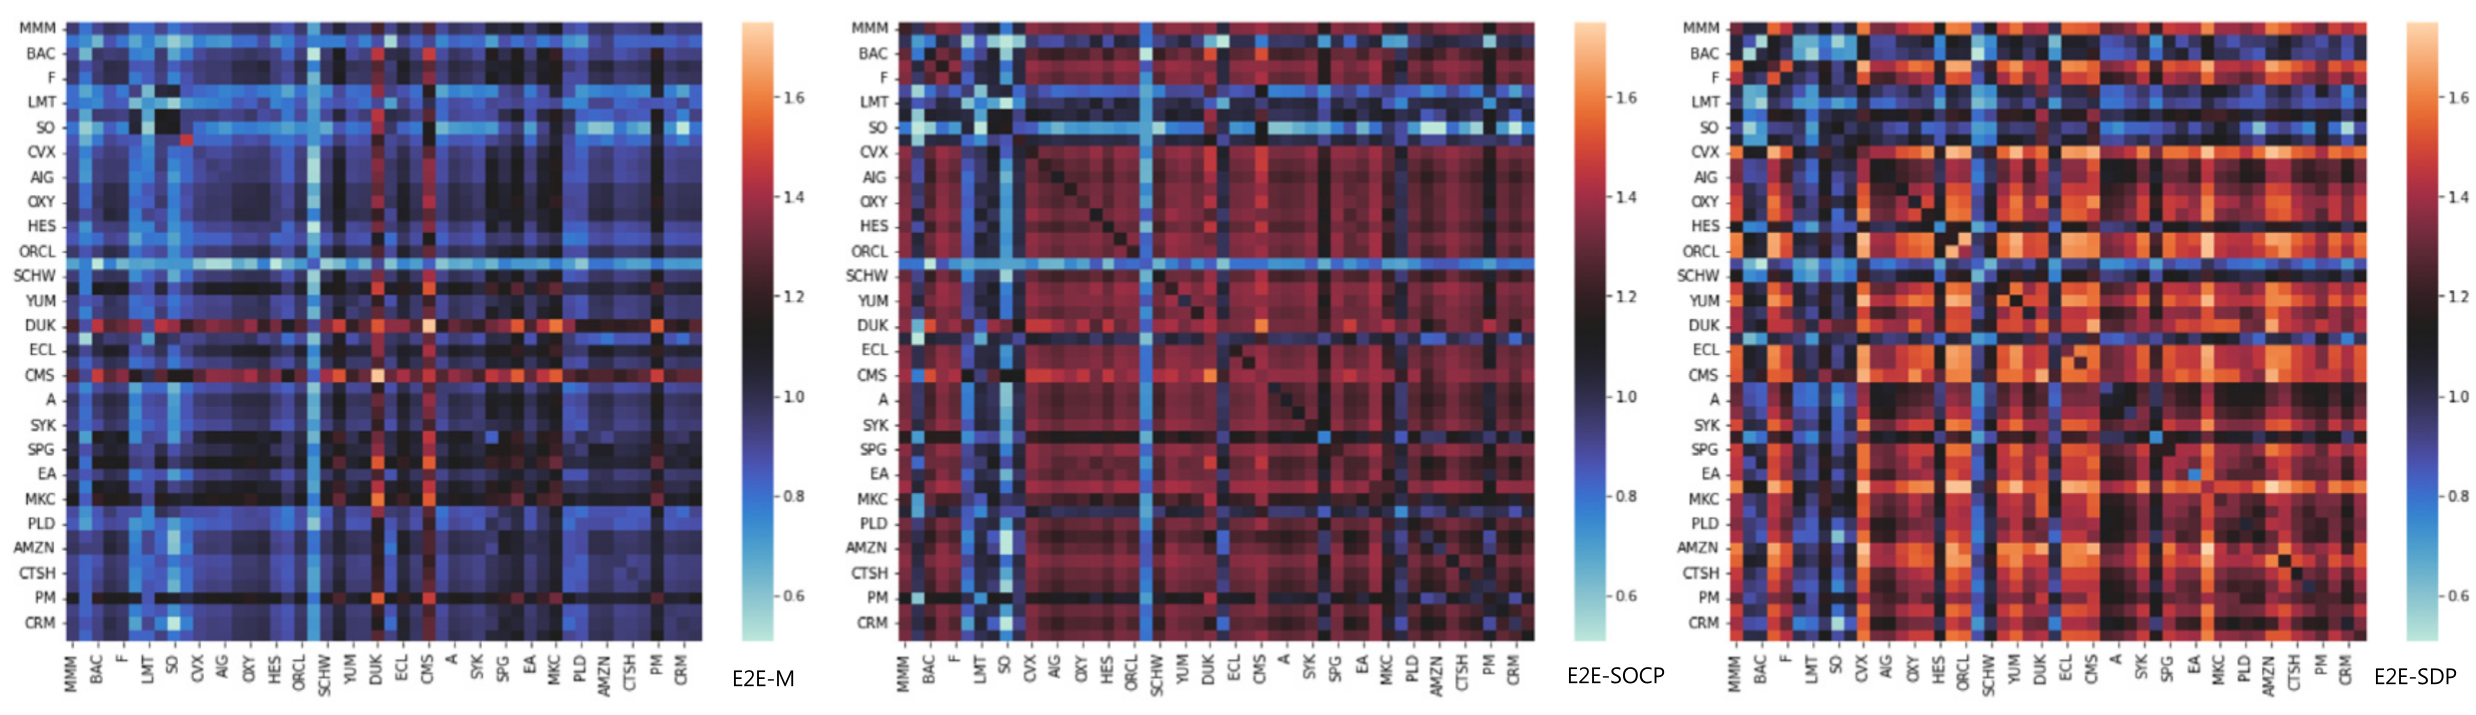
\includegraphics[width=\textwidth,height=.30\textheight,keepaspectratio]{fig3.png}
    \end{center}


  \item Training cost is not negligible.
  
    {\centering
    \vspace{0.2em}
    \scriptsize 
        \begin{tabular}{lcc}
    \toprule
    Layer & Structure & Reported epoch-time scale \\
    \midrule
    E2E $M$ & convex QP & about 15 seconds \\
    E2E SOCP & conic perspective constraints & about 1 minute \\
    E2E SDP & lifted semidefinite cone & over 6 hours \\
    \bottomrule
  \end{tabular}
    
    }

      \end{enumerate}

\end{frame}


\begin{frame}{In-sample result: E2E beats linReg}
  Across 24 training periods, the paper counts pairwise wins.

  \centering\small
  \begin{tabular}{lccc}
    \toprule
    Metric against linReg & $\Kcard=10$ & $\Kcard=15$ & $\Kcard=20$ \\
    \midrule
    E2E $M$ variance wins & $21/24$ & $19/24$ & $19/24$ \\
    E2E SOCP variance wins & $23/24$ & $21/24$ & $20/24$ \\
    E2E SDP variance wins & $21/24$ & $19/24$ & $19/24$ \\
    \midrule
    Any E2E return wins & $24/24$ & $24/24$ & $24/24$ \\
    Any E2E Sharpe wins & $24/24$ & $24/24$ & $24/24$ \\
    \bottomrule
  \end{tabular}

  \vspace{.8em}
  \begin{itemize}
    \item  The integrated learner improves in-sample returns and Sharpe ratios consistently, with little or no volatility penalty.
  \end{itemize}
\end{frame}

\begin{frame}{Appendix: out-of-sample metrics}
  \small
  \begin{tabular}{>{\raggedright\arraybackslash}p{.25\linewidth}p{.62\linewidth}}
    \toprule
    Metric & Interpretation \\
    \midrule
    Annualized return & geometric average return scaled to one year \\
    Annualized volatility & standard deviation of portfolio returns scaled by $\sqrt{256}$ \\
    VaR / CVaR & tail-loss measures at $\alpha=0.05$ \\
    LPM2 & second-order lower partial moment below zero return \\
    Max drawdown & largest peak-to-trough wealth decline \\
    Sharpe / Sortino / Calmar & risk-adjusted returns using volatility, downside risk, or drawdown \\
    Information ratio & active return over tracking error relative to nominal benchmark \\
    \bottomrule
  \end{tabular}
\end{frame}

\begin{frame}{Out-of-sample risk and return}
  \centering\footnotesize
  \begin{tabular}{llccccc}
    \toprule
    Metric & $\Kcard$ & E2E $M$ & E2E SOCP & E2E SDP & linReg & nominal \\
    \midrule
    Ann. ret. & 10 & .1908 & .1776 & .1699 & .1535 & .1684 \\
              & 15 & .1707 & .1697 & .1698 & .1424 & .1533 \\
              & 20 & .1729 & .1687 & .1708 & .1441 & .1550 \\
    \midrule
    Ann. vol. & 10 & .1674 & .1695 & .1697 & .1755 & .1686 \\
              & 15 & .1686 & .1667 & .1670 & .1701 & .1680 \\
              & 20 & .1687 & .1669 & .1682 & .1700 & .1674 \\
    \midrule
    Max DD    & 10 & .3149 & .3361 & .3331 & .3585 & .3417 \\
              & 15 & .3358 & .3347 & .3208 & .3491 & .3657 \\
              & 20 & .3357 & .3348 & .3370 & .3476 & .3632 \\
    \bottomrule
  \end{tabular}

  \vspace{.2em}
  {\scriptsize
  \begin{itemize}
    \item Every E2E variant has higher annualized return than linReg at all cardinalities.
    \item E2E also reduces annualized volatility relative to linReg.
    \item Compared with nominal, E2E has better return, volatility and maximum drawdown; however, nominal has better VaR and CVaR.
    \item Inside the E2E variants, Big-M has the best return and Sharpe, with also higher volatility.
  \end{itemize}
  }
\end{frame}

\begin{frame}{Out-of-sample risk-adjusted metrics}
  \centering\footnotesize
  \begin{tabular}{llccccc}
    \toprule
    Metric & $\Kcard$ & E2E $M$ & E2E SOCP & E2E SDP & linReg & nominal \\
    \midrule
    Sharpe & 10 & 1.1399 & 1.0014 & 1.0474 & .8747 & .9993 \\
           & 15 & 1.0126 & 1.0169 & 1.0180 & .8370 & .9128 \\
           & 20 & 1.0247 & 1.0155 & 1.0106 & .8478 & .9265 \\
    \midrule
    Sortino & 10 & 2.3407 & 2.0179 & 2.1009 & 1.6560 & 2.0171 \\
            & 15 & 2.0391 & 2.0677 & 2.0577 & 1.6301 & 1.7960 \\
            & 20 & 2.0606 & 2.0413 & 2.0420 & 1.6602 & 1.8397 \\
    \midrule
    Calmar & 10 & .6059 & .5102 & .5284 & .4280 & .4930 \\
           & 15 & .5083 & .5294 & .5071 & .4079 & .4193 \\
           & 20 & .5150 & .5068 & .5039 & .4145 & .4269 \\
    \bottomrule
  \end{tabular}
\vspace{.2em}
\begin{itemize}
  \item E2E is consistently significantly better than linReg, and also better than nominal.
  \item Compared with nominal, E2E brings positive extra return adjusted by risk, while linReg does the opposite.
\end{itemize}

\end{frame}

\section{Discussion}

\begin{frame}{Counterintuitive relaxation performance}
  \small 
  The original intuition from combinatorial optimization:
  \[
    \text{tighter relaxation}
    \quad\Rightarrow\quad
    \text{better surrogate}
    \quad\Rightarrow\quad
    \text{better decisions}.
  \]

  The paper's evidence is more complicated:
  \begin{itemize}
    \item E2E $M$ often posts the strongest out-of-sample risk-adjusted performance.
    \item SOCP and SDP can reduce volatility, but do not clearly dominate in returns.
    \item The tighter layers are far more expensive and have larger optimization architectures.
  \end{itemize}

\end{frame}



% \begin{frame}{What the paper demonstrates well}
%   \begin{itemize}
%     \item A concrete recipe for making sparse portfolio optimization differentiable enough for end-to-end training.
%     \item A clean distinction between prediction accuracy and realized portfolio quality.
%     \item Evidence that integrated factor-model learning can correct biases relevant to the downstream sparse optimizer.
%     \item A useful warning that ``tighter relaxation'' is not a universal proxy for ``better learning layer''.
%   \end{itemize}
% \end{frame}

% \begin{frame}{Limitations to keep visible}
%   \begin{enumerate}
%     \item The gradient is taken through relaxations, while test-time portfolio construction solves the original Big-M MIP.
%     \item The data universe is practical but small: $\Nassets=50$.
%     \item The training instances are synthetic CBB samples, so results depend on bootstrap design.
%     \item Transaction costs are reported via turnover but not built into the training objective.
%     \item The loss is realized Sharpe, which is noisy and path-dependent.
%   \end{enumerate}
% \end{frame}


\begin{frame}{References}
  \begingroup
  \renewcommand*{\bibfont}{\scriptsize}
  \setlength{\bibitemsep}{0.2\baselineskip}
  \setlength{\bibparsep}{0pt}
  \setlength{\bibhang}{1.2em}
  \setlength{\biblabelsep}{0.45em}
  \printbibliography[heading=none]
  \endgroup
\end{frame}

\end{document}
